\documentclass[11pt,a4paper]{article}
\usepackage[a4paper,hmargin=1in,vmargin=1in]{geometry}
\usepackage{pgfplots}
\pgfplotsset{compat=1.17}

\usepackage[czech]{babel}
\usepackage[utf8]{inputenc}
\usepackage[T1]{fontenc}

\usepackage[nodayofweek]{datetime}
\newdate{date}{14}{6}{2023}

\usepackage{stddoc}
\usepackage{lipsum}
\usepackage{subcaption}

\newcommand{\plus}{{\texttt{+}}}
\renewcommand{\Re}{\operatorname{Re}}
\renewcommand{\Im}{\operatorname{Im}}
\newcommand{\fourier}[3]{\mathcal{F}_{#1}\!\left[#2\right]\!\left(#3\right)}
\newcommand{\ifourier}[3]{\mathcal{F}^{-1}_{#1}\!\left[#2\right]\!\left(#3\right)}
\newcommand{\dB}{\mathrm{dB}}
\newcommand{\dBm}{\mathrm{dBm}}
\newcommand{\MHz}{\mathrm{MHz}}
\newcommand{\GHz}{\mathrm{GHz}}
\newcommand{\kHz}{\mathrm{kHz}}


\begin{document}

\pagenumbering{arabic}

% Header
\begin{center}
    {\LARGE\textbf{Laboratorní úloha č. 7}}\\[3mm]
    \begin{minipage}{0.4\textwidth}
        \begin{flushleft}
            \textsc{\displaydate{date}}
        \end{flushleft}
    \end{minipage}
    ~
    \begin{minipage}{0.4\textwidth}
        \begin{flushright}
            \textsc{Martin Šimák}
        \end{flushright}
    \end{minipage}
    \noindent\rule{14.5cm}{0.4pt}
\end{center}

\paragraph*{Měření velkosignálových vlastností mikrovlnných směšovačů a násobičů} Laboratorní úloha ukazuje možnosti měření mikrovlnného výkonu termálním a diodovým detektorem a vysílaného pulzního radarového senzoru.

\subsection*{Úkoly měření}
\begin{enumerate}
    \item Měření dodaného výkonu do záteže přes směrovou odbočnici
    \item Měření efektivního vysílaného isotropického výkonu (EIRP) radaru
\end{enumerate}

\subsection*{Použité přístroje a komponenty}
\begin{itemize}
    \item Spektrální analyzátor R\&S FSW26 (2~Hz až 26,5~GHz)
    \item Harmonický mixér R\&S FS-Z90 (60~GHz až 90~GHz)
    \item Trychtýřová anténa RFspin H-A90-W25 (60~GHz až 90~GHz)
    \item Detektor R\&S NRP40TN (DC až 40~GHz)
    \item Detektor Giga-tronics 80401A (0.01~MHz až 18~GHz)
    \item Vyhodnocovací jednotka detektoru Giga-tronics 8541C
    \item Generátor ELSY SG3000 (100~kHz až 3~GHz)
    \item Nízkofrekvenční generátor RIGOL DG2041A (do 40~MHz)
    \item Směrová odbočnice Tesla CGN 102 10 (1~GHz až 2~GHz)
    \item Dělič výkonu Mini-Circuits ZX10-2-20-S\plus\ (200~MHz až 2~GHz)
    \item Integrovaná milimetrová jednotka (IMJ)
    \item Generátor Agilent E8257D (250~kHz až 50~GHz)
    \item Kabely s N konektorem (Pasternack PE302-24)
    \item Propojovací SMA kabely
\end{itemize}

\subsection*{Měřené komponenty}
\begin{itemize}
    \item Radarový modul Texas Instruments AWR1642BOOST (77~GHz až 81~GHz)
\end{itemize}

\subsection*{Popis měření}

% Task 1
\paragraph*{Porovnání možností diodového a termálního detektoru - demonstrace} Měření probíhalo dle schématu zapojení na obrázku~\ref{fig:task1-zapojeni}, kde generátor Rigol slouží jako generátor ASK modulačního signálu, generátor ELSY produkuje modulovaný harmonický signál o frekvenci 1~GHz a spektrální analyzátor slouží pouze jako jednotka pro zobrazování výkonů naměřených na detektorech R\&S (termální) a Giga-tronics (diodový).
\begin{figure}[!ht]
    \centering
    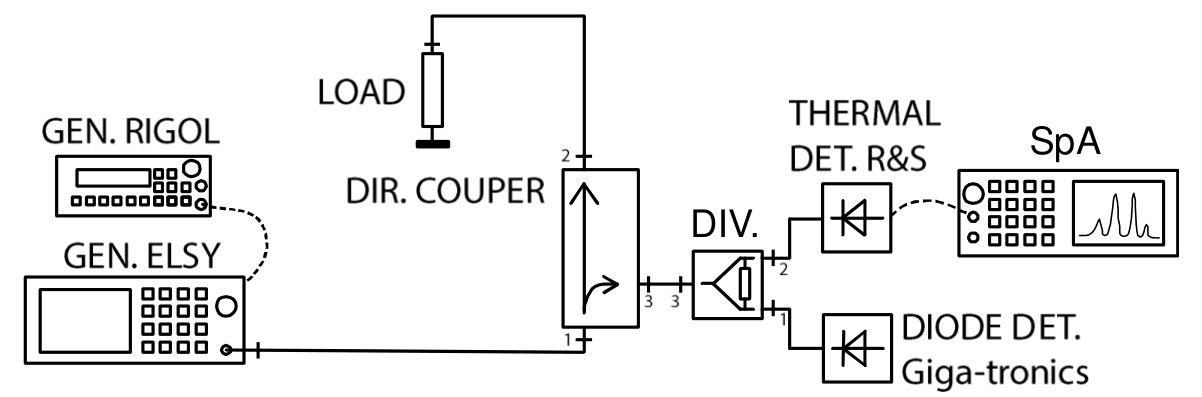
\includegraphics[width=.8\textwidth]{src/task1-zapojeni.png}
    \caption{\label{fig:task1-zapojeni}Schéma zapojení úlohy}
\end{figure}
V rámci měření bylo demonstrováno, že zatímco pro měření nemodulovaného signálu jsou možnosti obou detektorů srovnatelné, po zapnutí ASK modulace umožňuje diodový detektor oproti termálnímu více flexibility. Termální detektor totiž vykazuje pouze průměrnou hodnotu výkonu $-10+10\log(0.05)\ \dBm$, kde $-10\ \dBm$ je výkon nemodulovaného signálu generátoru ELSY a $0.05$ je střída modulačního ASK signálu, kdežto diodový detektor umožňuje díky rychlejší reakci na změnu výkonové hladiny signálu analyzovat i pulzy s náhodnou periodou a délkou (režim \emph{Burst Avg}). Krom toho diodový detektor umožňuje též změřit i překmit výkonu v pulzu oproti průměrné hodnotě výkonu v pulzu, neboli tzv. \emph{crest factor}. Tento faktor je ovlivněn jak překmity, tak i rychlostí hran pulzu.

% Task 2
\paragraph*{Měření dodaného výkonu do zátěže přes směrovou odbočnici} Cílem této úlohy bylo ukázat, jak lze měřit výkon dodaný do zátěže nepřímo přes směrovou odbočnici. Ve vysílací technice, kde jsou k anténě dodávány minimálně jednotky wattů výkonu, nelze často měřit výkon přímo, protože běžné mikrovlnné detektory nemají dostatečně velký rozsah měřených výkonů. Zároveň se vysílaný výkon průběžně monitoruje a je součástí smyčky ALC (automatic leveling control). Schéma zapojení úlohy je na obrázku~\ref{fig:task2-zapojeni}.
\begin{figure}[!ht]
    \centering
    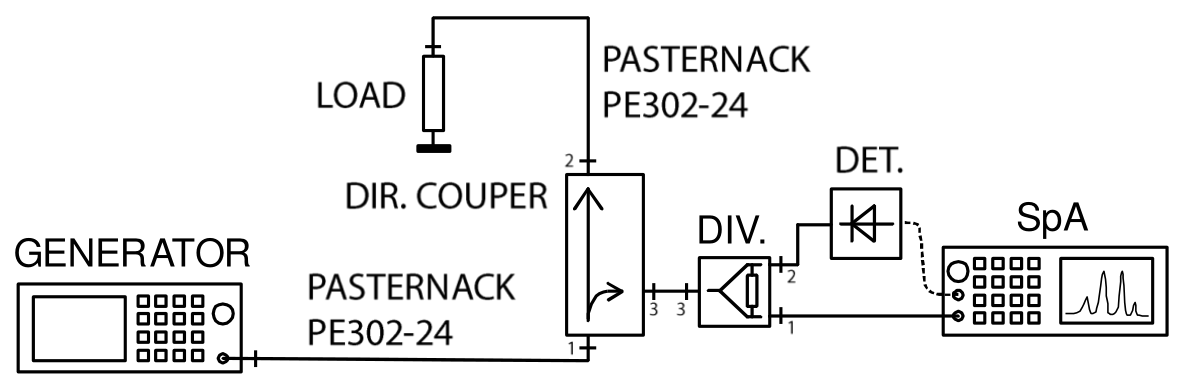
\includegraphics[width=.8\textwidth]{src/task2-zapojeni.png}
    \caption{\label{fig:task2-zapojeni}Schéma zapojení úlohy}
\end{figure}

V této úloze slouží spektrální analyzátor jako zobrazovací jednotka pro výkon měřený termálním detektorem a dále detektor informuje o frekvenci vysílaného signálu. Do zátěže se vysílá jen CW signál. Nastavení přístrojů:
\begin{itemize}
    \item vypnutá modulace ASK generátoru,
    \item frekvence výstupního signálu generátoru na 1~GHz a výkon 0~dBm,
    \item spektrální analyzátor s frekvenčním rozsahem měření od 0.9~GHz do 2.1~GHz, jinak v základním nastavení,
    \item svižné měření detektoru s korekcí změřené hodnoty výkonu podle měření frekvence z interních kalibračních dat (\emph{Continuous Update: On}, \emph{Frequency Coupling: Marker}).
\end{itemize}
Po zapnutí detektoru (\emph{Power Sensor Config -- State: On}) a nastavení markeru tak, aby vždy sledoval špičku s nejvyšším měřeným výkonem (\emph{Marker Config -- Auto Max Peak: On}), na generátoru postupně měníme frekvenci signálu v rozsahu 1~GHz až 2~GHz, tedy v rozsahu funkčnosti směrové odbočnice, a výkony $P_{\mathrm{DET}}$ změřené detektorem jsou zaznamenány v tabulce~\ref{table:task2-data}.
\begin{table}[!ht]
    \centering
    \begin{tabular}{|l||c|c|c|c|c|c|c|c|c|c|}
        \rule{2cm}{0pt} & \rule{1.5cm}{0pt} & \rule{1.5cm}{0pt} & \rule{1.5cm}{0pt} & \rule{1.5cm}{0pt} & \rule{1.5cm}{0pt}\\[-\arraystretch\normalbaselineskip]
        \hline
        $f\ [\mathrm{MHz}]$ & 1100 & 1200 & 1300 & 1400 & 1500\\
        \hline
        $P_{\mathrm{DET}} \ [\mathrm{dBm}]$ & -17.52 & -17.57 & -17.76 & -17.78 & -17.91\\
        \hline
        $P_{\mathrm{LOAD}} \ [\mathrm{dBm}]$ & -5.58 & -5.66 & -5.83 & -5.78 & -5.84\\
        \hline\hline
        $f\ [\mathrm{MHz}]$ & 1600 & 1700 & 1800 & 1900 & 2000\\
        \hline
        $P_{\mathrm{DET}} \ [\mathrm{dBm}]$ & -17.87 & -18.14 & -18.31 & -18.35 & -18.80\\
        \hline
        $P_{\mathrm{LOAD}} \ [\mathrm{dBm}]$ & -5.73 & -6.00 & -6.08 & -5.98 & -6.09\\
        \hline
    \end{tabular}
    \caption{\label{table:task2-data}Naměřené a vypočítané hodnoty výkonu}
\end{table}

Výkon změřený přes směrovou odbočnici není ten, který je dodáván do zátěže. K dispozici máme změřené S-parametry dvou stejných kabelů Pasternack, použité směrové odbočnice a děliče výkonu. V programu AWR lze tak jednoduše sestavit obvod z bloků S-parametrů jako na obrázku~\ref{fig:task2-sparametry}.
\begin{figure}[!ht]
    \centering
    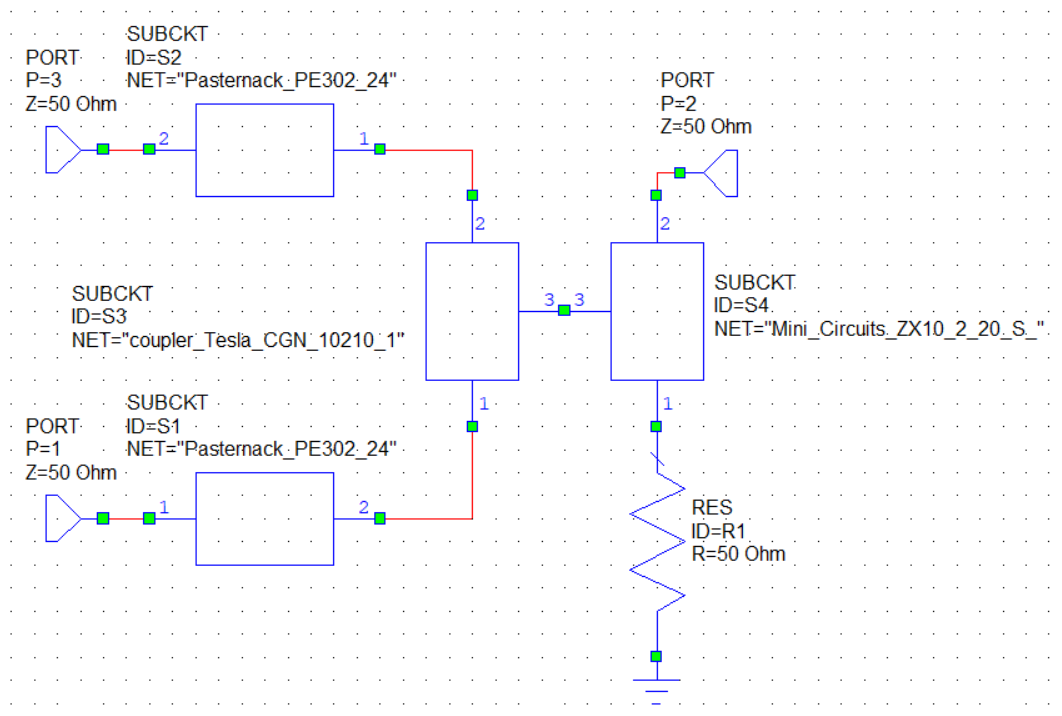
\includegraphics[width=.8\textwidth]{src/task2-sparametry.png}
    \caption{\label{fig:task2-sparametry}Schéma sestavené z bloků S-parametrů}
\end{figure}
Měření výkonu $P_{\mathrm{DET}}$ bylo provedeno v místě portu 2 a předpokládáme, že vstup spektrálního analyzátoru i detektor byly bezodrazové. Ze známého výkonu generátoru $P_{\mathrm{in}}$ se dá detekovaný výkon spočítat jako
\begin{align}
    P_{\mathrm{DET}} = P_{\mathrm{in}} \left|S_{21}\right|.
\end{align}
Výkon dodávaný do zátěže se dá pak spočítat jako
\begin{align}
    P_{\mathrm{LOAD}} = P_{\mathrm{in}} \left|S_{31}\right| = P_{\mathrm{DET}} \frac{\left|S_{31}\right|}{\left|S_{21}\right|},
\end{align}
tedy bez potřeby znát skutečnou hodnot výkonu $P_{\mathrm{in}}$ generovaného signálu. Hodnoty $P_{\mathrm{LOAD}}$ v tabulce~\ref{table:task2-data} jsme získali touto metodou, kde S-parametry byly získány simulací obvodu~\ref{fig:task2-sparametry}. Grafy těchto hodnot jsou znázorněny na obrázku~\ref{fig:task2-sparameter-data}.
\begin{figure}[!ht]
    \centering
    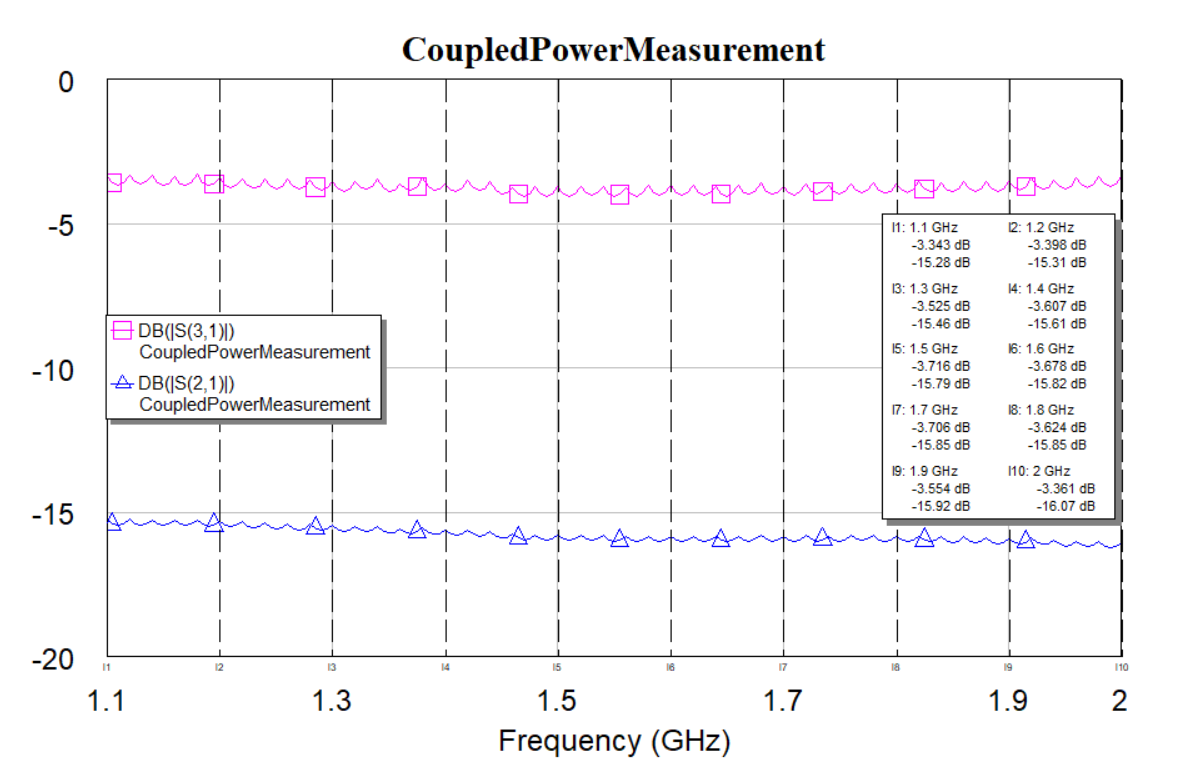
\includegraphics[width=.8\textwidth]{src/task2-sparameter_data.png}
    \caption{\label{fig:task2-sparameter-data}S-parametry soustavy odbočující měřený výkon}
\end{figure}

% Task 3
\paragraph*{Měření harmonického signálu pomocí harmonického mixéru - demonstrace} Zapojení úlohy je patrné z obrázku~\ref{fig:task3-zapojeni}. Spektrální analyzátor má na vstupu připojen harmonický mixér, který přes anténu na vlnovodu WR-12 přijímá signály ve frekvenčním pásmu 60~GHz až 90~GHz.
\begin{figure}[!ht]
    \centering
    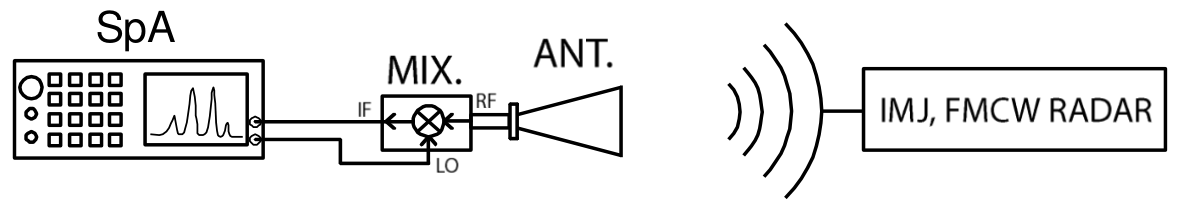
\includegraphics[width=0.8\textwidth]{src/task3-zapojeni.png}
    \caption{\label{fig:task3-zapojeni}Schéma zapojení úlohy}
\end{figure}
Pro měření byly přístroje v následujícím nastavení:
\begin{itemize}
    \item mixér zapnut a nastaven jako 3-port v pracovním pásmu E (60~GHz až 90~GHz) pro detekci harmonických složek 6. řádu,
    \item do mixéru vpuštěn signál LO ze spektrálního analyzátoru o výkonové hladině 14 dBm jako při kalibraci výrobcem,
    \item zapnutá identifikace zrcadlových příjmů.
\end{itemize}
Zdrojem harmonického signálu o frekvenci 82~GHz je \emph{integrovaná milimetrová jednotka} (IMJ) sestávající ze směšovače a antény. IMJ je na vstupu LO buzena z generátoru Agilent signálem o frekvenci 41~GHz a dojde v ní ke zdvojnásobení této frekvence. Na vstupu IF není připojeno nic, a tak z antény IMJ se vysílá pouze prosakující signál LO.

Spektrální analyzátor posílá do vstupu LO mixéru silný signál o frekvenci $f_{\mathrm{LO}}/n$, kde $n=6$, a přijímá mezifrekvenční signál IF na frekvenci $f_{\mathrm{IF}} = 1300\ \MHz$. Spektrální analyzátor jakožto heterodynní přijímač obecně přijímá všechny RF signály splňující relaci $|nf_{\mathrm{LO}}\pm f_{\mathrm{RF}}| = f_{\mathrm{IF}}$, kde $n \in \N$. V běžném režimu spektrální analyzátor používá frekvenci $f_{\mathrm{LO}} = (f_{\mathrm{RF}}+f_{\mathrm{IF}})/6$, tj. $f_{\mathrm{LO}} \in \{10.22\ \GHz,15.22\ \GHz\}$. Pro identifikaci zrcadlového příjmu je ale střídavě používána i frekvence $f_{\mathrm{LO}} = (f_{\mathrm{RF}} - f_{\mathrm{IF}})/6$, tj. $f_{\mathrm{LO}} \in \{9.78\ \GHz, 14.78\ \GHz\}$.

Ve změřeném spektru se bez automatické detekce falešných příjmů zobrazuje hned několik harmonických signálů. Na směšovači se díky silně přebuzené nelinearitě vytvoří i další harmonicé složky LO signálu a dojde ke směšování všech harmonických složek LO se vstupním RF signálem. Na spektrálním analyzátoru lze vidět příjem signálů $f_{\mathrm{RF}}$ a $f_{\mathrm{RF}}\pm2f_{\mathrm{IF}}$.

Po nasatvení automatického potlačování falešných příjmů (\emph{Auto ID} na \emph{On}) zůstává vidět jen signál $f_{\mathrm{RF}}$. Tato selekce je prováděna na základě toho, že jakmile je nějaký signál detekován v obou variantách příjmu, je považován za reálný.

% Task 4
\paragraph*{Měření EIRP radaru} Zapojení je ponecháno z předchozí úlohy, tj. zapojení na obrázku~\ref{fig:task3-zapojeni}. Zdrojem signálu je nyní radarový modul TI AWR1642BOOTS.

Měření je třeba provádět ve vzdálené zóně vyzařování, k čemuž využijeme známý vzorec z teorie antén pro aproximaci hranice Fraunhoferovy zóny
\begin{align}
    \label{eq:farfield}
    d_{\mathrm F} = \frac{2D^2}{\lambda} = \frac{2D^2f}{c},
\end{align}
kde $D$ je nejdelší rozměr apertury vysílací antény -- v našem případě diagonála trychtýře -- a $c$ je rychlost světla. Tato hodnota $d_{\mathrm F}$ je pro nejvyšší měřenou frekvenci 80.9~GHz rovna zhruba 82~cm. S jistou rezervou jsme tedy zvolili výslednou vzdálenost $d = 86.5\ \mathrm{cm}$.

Samotné měření probíhá zapomoci markerů umístěných na okrajích pásma radarového signálu 77~GHz a 81~GHz, s frekvenčním rozsahem 76~GHz až 82~GHz%
    \footnote{Prohlížíme-li si spektrum, které analyzátor měří standardně v celém pásmu 60~GHz až 90~GHz, můžeme pozorovat téměř všude občasně detekované části radarem vysílaných čirpů. Jelikož totiž signál přijímáme harmonickým mixérem, přijímané RF frekvence mohou po směšování obecně s $n$-tou harmonickou na frekvenci $nf_{\mathrm{LO}}$ padnout do mezifrekvenčního pásma, což vede na detekci frekvenčně posunuté \uv{kopie} přijímaného signálu.}
a nastavením sweepu přes pásmo trvající 1~s. Přes toto měření je vhodné dále nastavit trace, která si bude pamatovat maximum přijatého výkonu (\emph{Trace Mode} na \emph{Max Hold, Detector Positive Peak}).

Pomocí nastaveného markeru s volbou \emph{Marker to Trace} je možné odečítat přijatý výkon $P_{\mathrm{RX}}$ a z něho následně spočítat $\mathit{EIRP}$ radaru pomocí Friisovy přenosové rovnice jako
\begin{align}
    \mathit{EIRP} = P_{\mathrm{TX}} + G = P_{\mathrm{RX}} + \mathit{FSL} - 2G + G = P_{\mathrm{RX}} + \mathit{FSL} - G
\end{align}
kde $G = 25\ \dB$ je zisk použité antény a $\mathit{FSL}$ jsou ztráty volným prostorem, pro něž platí
\begin{align}
    \mathit{FSL} = 20\log\(\frac{4\pi d}{\lambda}\)\ \dB.
\end{align}
Takto naměřené a následně zpracované výsledky jsou k nahlédnutí v tabulce~\ref{table:task4-data}.
\begin{table}[!ht]
    \centering
    \begin{tabular}{|l||c|c|c|c|c|}
        \rule{2cm}{0pt} & \rule{1cm}{0pt} & \rule{1cm}{0pt} & \rule{1cm}{0pt} & \rule{1cm}{0pt} & \rule{1cm}{0pt}\\[-\arraystretch\normalbaselineskip]
        \hline
        $f \ [\mathrm{GHz}]$ & 77.1 & 78 & 79 & 80 & 80.9\\
        \hline
        $P_{\mathrm{RX}} \ [\mathrm{dBm}]$ & -25.59 & -26.03 & -24.73 & -22.59 & -23.41\\
        \hline
        $\mathit{FSL} \ [\mathrm{dB}]$ & 68.9 & 69.0 & 69.1 & 69.2 & 69.3\\
        \hline\hline
        $\mathit{EIRP} \ [\mathrm{dBm}]$ & 18.3 & 18.0 & 19.4 & 21.7 & 20.9\\
        \hline
    \end{tabular}
    \caption{\label{table:task4-data}Naměřená a vypočítaná data}
\end{table}

% Task 5
\paragraph*{Měření rychlých dějů pomocí real-time spektra - demonstrace} Tato úloha sloužila k demonstraci možnosti spektrálního analyzátoru vzorkovat signál s šířkou pásma 160~MHz. Z těchto vzorků v časové oblasti lze pak vypočítat spektrum pomocí Fourierovy transformace a zobrazit spektrum přijatého signálu. Tímto způsobem lze detekovat i rychlé děje, které by přelaďovaný heterodynní přijímač změřil jen náhodou.


\subsection*{Závěr}
V rámci laboratorní úlohy jsme se seznámili s možnostmi měření mikrovlnných výkonů, a to jak výkonu přenášeného po vedení pomocí termálního a diodového detektoru, tak i výkonu vysílaného pulzním radarovým senzorem. Měření proběhlo bez výraznějších potíží, a byli jsme tak schopni si vyzkoušet metody, které nám byly teoreticky uvedeny na přednáškách.


\end{document}
